\documentclass{article}
%\usepackage[francais]{babel}
%\usepackage[utf8]{inputenc} % Required for including letters with accents
%\usepackage[T1]{fontenc} % Use 8-bit encoding that has 256 glyphs
\usepackage{pythontex}
\usepackage{amsthm}
\usepackage{amsmath}
\usepackage{amssymb}
\usepackage{mathrsfs}
\usepackage{graphicx}
\usepackage{geometry}
\usepackage{stmaryrd}
\usepackage{tikz}
\usetikzlibrary{patterns}
%\usetikzlibrary{intersections}
\usepackage[cache=false]{minted}
\usepackage{xcolor}

\usepackage{stmaryrd}
%\usetikzlibrary{tikzmark}
\usepackage{empheq}
\usepackage{longtable}
\usepackage{booktabs} 
\usepackage{array}
\usepackage{pstricks}
\usepackage{pst-3dplot}
\usepackage{pst-tree}
\usepackage{pstricks-add}
\usepackage{upgreek}
%\usepackage{epstopdf}
\usepackage{eolgrab}
\usepackage{chngpage}
 \usepackage{calrsfs}
 % Appel du package pythontex 
\usepackage{pythontex}

\usepackage{algorithm2e}
\RestyleAlgo{algoruled}
  \SetKw{KwFrom}{from} 
\newenvironment{algo}{
\begin{algorithm}[H]
\DontPrintSemicolon \SetAlgoVlined}
{\end{algorithm}}



\usetikzlibrary{decorations.pathmorphing}
\def \de {{\rm d}}
\usepackage{color}
\usepackage{xcolor}
\newcommand{\mybox}[1]{\fbox{$\displaystyle#1$}}
\newcommand{\myredbox}[1]{\fcolorbox{red}{white}{$\displaystyle#1$}}
\newcommand{\mydoublebox}[1]{\fbox{\fbox{$\displaystyle#1$}}}
\newcommand{\myreddoublebox}[1]{\fcolorbox{red}{white}{\fcolorbox{red}{white}{$\displaystyle#1$}}}

\usepackage{xcolor}
%\setbeamercolor{background canvas}{bg=lightgray}
\definecolor{LightGray}{gray}{0.9}
\definecolor{monOrange}{rgb}{0.97,0.35,0.04}
\usepackage{enumitem}
 \title{Le style et les classes}
\author{Ibrahim ALAME}
\date{14/02/2023}
\begin{document}
\maketitle

\section{Introduction et portée des styles}
\subsection{Comportement par défaut}
Par défaut, tout le CSS est global car il est réuni dans le {\color{monOrange}bundle} par {\color{monOrange}Vite}. Si vous définissez des classes à l'intérieur des balises {\tt <style>}, ces classes s'appliqueront donc à tous vos composants.

\subsection{L'attribut {\color{monOrange}scoped}}
L'attribut {\color{monOrange}scoped} permet d'encapsuler le CSS d'un composant monofichier ({\color{monOrange}SFC}) en ajoutant, grâce à PostCSS un attribut unique (par exemple data-v-29e5g83) à l'élément en compilant par exempl {\color{monOrange}.ma-classe} en {\color{monOrange}.ma-classe[data-v-29e5g83]}.

Cette encapsulation est effectuée automatiquement par {\color{monOrange}Vite}. Vous n'avez rien à faire d'autre que d'ajouter l'attribut {\color{monOrange}scoped}. Pour utiliser {\color{monOrange}scoped}, il suffit de l'ajouter sur la balise style de votre composant monofichier :
\begin{minted}[
mathescape,
framesep=2mm,
baselinestretch=1.2,
%fontsize=\footnotesize,
bgcolor=LightGray,
%linenos
]{html}
<style scoped>
  .ma-classe {
  }
</style>
\end{minted}

%Exemple exécutable de la vidéo
%Vous pouvez directement utiliser ce code exécutable. N'hésitez pas à l'ouvrir dans un nouvel onglet pour le modifier ou mieux voir :

\section{La liaison de classes}
\subsection{La liaison de classes}
Nous avons vu qu'il était possible de lier une ou plusieurs classes à l'attribut {\color{monOrange}class} en utilisant la directive {\color{monOrange}v-bind}. Pour permettre une utilisation très flexible, {\color{monOrange}Vue.js} permet plus de syntaxes lorsque nous utilisons {\color{monOrange}v-bind} avec les classes ou les styles.

Bien sûr la liaison n'a de sens que si les classes sont réactives suivant la valeur de propriétés. Sinon il suffit d'écrire les classes en dur côté {\color{monOrange}template}. Nous allons récapituler toutes les syntaxes possibles.

\subsubsection{Liaison avec des objets}
La première syntaxe permet d'utiliser un objet :
\begin{minted}[
mathescape,
framesep=2mm,
baselinestretch=1.2,
%fontsize=\footnotesize,
bgcolor=LightGray,
%linenos
]{html}
<div :class="{ actif: estActif }"></div>
\end{minted}
La classe {\color{monOrange}actif} sera ajoutée si la propriété {\tt estActif} vaut {\tt true} :
\begin{minted}[
mathescape,
framesep=2mm,
baselinestretch=1.2,
%fontsize=\footnotesize,
bgcolor=LightGray,
%linenos
]{javascript}
const estActif = ref(true)
\end{minted}
Si la propriété réactive passe à {\tt false}, la classe sera automatiquement retirée.

\subsubsection{Combinaison de l'attribut {\color{monOrange}class} et d'une liaison {\color{monOrange}:class}}
Vous pouvez combiner sans problème l'attribut {\color{monOrange}class} avec une liaison avec la directive {\color{monOrange}v-bind} en utilisant {\color{monOrange}:class} :
\begin{minted}[
mathescape,
framesep=2mm,
baselinestretch=1.2,
%fontsize=\footnotesize,
bgcolor=LightGray,
%linenos
]{html}
<div
  class="classe1"
  :class="{ active: isActive, error: hasError }"
></div>
\end{minted}
Ici nous aurons quoiqu'il arrive la {\tt classe1}.
\begin{itemize}
\item La classe {\color{monOrange}active} sera ajoutée si la propriété {\color{monOrange}isActive} vaut {\tt true}.
\item La classe {\color{monOrange}error} sera ajoutée si la propriété {\color{monOrange}hasError} vaut {\tt true}.
\end{itemize}
Dans tous les cas, Vue.js créera la div sur le DOM avec un seul attribut classe, par exemple :
\begin{minted}[
mathescape,
framesep=2mm,
baselinestretch=1.2,
%fontsize=\footnotesize,
bgcolor=LightGray,
%linenos
]{html}
<div class="classe1 isActive hasError"></div>
\end{minted}

\subsubsection{Utilisation d'un objet réactif}
Vous pouvez utiliser un objet réactif côté {\color{monOrange}script} pour la liaison avec l'attribut {\color{monOrange}class} :
\begin{minted}[
mathescape,
framesep=2mm,
baselinestretch=1.2,
%fontsize=\footnotesize,
bgcolor=LightGray,
%linenos
]{javascript}
const mesClasses = reactive({
  active: true,
  error: false,
  classeX: false
});
\end{minted}
Il suffit ensuite de le passer à {\color{monOrange}v-bind} :
\begin{minted}[
mathescape,
framesep=2mm,
baselinestretch=1.2,
%fontsize=\footnotesize,
bgcolor=LightGray,
%linenos
]{html}
<div :class="mesClasses"></div>
\end{minted}

\subsubsection{Utilisation d'une propriété calculée}
Vous pouvez même utiliser une propriété calculée :
\begin{minted}[
mathescape,
framesep=2mm,
baselinestretch=1.2,
%fontsize=\footnotesize,
bgcolor=LightGray,
%linenos
]{javascript}
const mesClasses = computed(() => ({
  active: isActive.value && !error.value,
  error: error.value && error.value.type === 'fatal'
}))
\end{minted}


\subsubsection{Utilisation d'un tableau de classes}
Vous pouvez utiliser un tableau de classes :
\begin{minted}[
mathescape,
framesep=2mm,
baselinestretch=1.2,
%fontsize=\footnotesize,
bgcolor=LightGray,
%linenos
]{html}
<div :class="[classe1, classe2]"></div>
\end{minted}

%Exemple exécutable de la vidéo
%Vous pouvez directement utiliser ce code exécutable. N'hésitez pas à l'ouvrir dans un nouvel onglet pour le modifier ou mieux voir :

\section{La liaison de styles}
\subsection{Liaison de styles}
Passons maintenant aux différentes syntaxes possibles pour les liaisons de style.

\subsubsection{Liaison avec des objets}
La première syntaxe permet d'utiliser un objet :
\begin{minted}[
mathescape,
framesep=2mm,
baselinestretch=1.2,
%fontsize=\footnotesize,
bgcolor=LightGray,
%linenos
]{html}
<div :style="{ color: activeColor, fontSize: fontSize + 'px' }"></div>
\end{minted}

Avec côté {\color{monOrange}script} :
\begin{minted}[
mathescape,
framesep=2mm,
baselinestretch=1.2,
%fontsize=\footnotesize,
bgcolor=LightGray,
%linenos
]{javascript}
const activeColor = ref('red')
const fontSize = ref(30)
\end{minted}

\subsubsection{Utilisation des propriétés CSS natives}
Vous pouvez également utiliser directement les noms des propriétés CSS en utilisant des guillemets simples :
\begin{minted}[
mathescape,
framesep=2mm,
baselinestretch=1.2,
%fontsize=\footnotesize,
bgcolor=LightGray,
%linenos
]{html}
<div :style="{ 'font-size': fontSize + 'px' }"></div>
\end{minted}

\subsubsection{Utilisation d'un objet réactif}
Vous pouvez utiliser un objet réactif côté script pour la liaison avec l'attribut {\color{monOrange}style} :
\begin{minted}[
mathescape,
framesep=2mm,
baselinestretch=1.2,
%fontsize=\footnotesize,
bgcolor=LightGray,
%linenos
]{javascript}
const mesStyles = reactive({
  color: 'red',
  fontSize: '13px'
})
\end{minted}
Et côté {\color{monOrange}template} :
\begin{minted}[
mathescape,
framesep=2mm,
baselinestretch=1.2,
%fontsize=\footnotesize,
bgcolor=LightGray,
%linenos
]{html}
<div :style="mesStyles"></div>
\end{minted}

\subsubsection{Utilisation d'un tableau}
Vous pouvez enfin utiliser un tableau :
\begin{minted}[
mathescape,
framesep=2mm,
baselinestretch=1.2,
%fontsize=\footnotesize,
bgcolor=LightGray,
%linenos
]{html}
<div :style="[stylesDeBase, stylesParticuliers]"></div>
\end{minted}
Ici les styles contenus dans l'objet {\color{monOrange}stylesDeBase} seront appliqués. Ensuite les styles contenus dans l'objet {\color{monOrange}stylesParticuliers} seront fusionnés. Si certaines propriétés sont dans les deux objets, les valeurs du dernier objet écraseront les valeurs précédentes.

Autrement dit, si par exemple il y a {\tt color:'red'} dans {\color{monOrange}stylesDeBase} et {\tt color:'blue'} dans {\color{monOrange}stylesParticuliers}. La valeur de la propriété {\tt color} sera {\tt blue}.

%Exemple exécutable de la vidéo
%Vous pouvez directement utiliser ce code exécutable. N'hésitez pas à l'ouvrir dans un nouvel onglet pour le modifier ou mieux voir :

\section{Utilisation de {\color{monOrange}Sass}}
L'utilisation de {\color{monOrange}Sass} avec {\color{monOrange}Vite} et {\color{monOrange}Vue.js} est extrêmement simple. Il suffit d'installer {\color{monOrange}sass} :
\begin{minted}[
mathescape,
framesep=2mm,
baselinestretch=1.2,
%fontsize=\footnotesize,
bgcolor=LightGray,
%linenos
]{bash}
npm add -D sass
\end{minted}
Et dans les composants {\color{monOrange}SFC} de préciser, comme pour {\color{monOrange}TypeScript} côté {\color{monOrange}template}, que les styles sont écrits en {\color{monOrange}Sass} :
\begin{minted}[
mathescape,
framesep=2mm,
baselinestretch=1.2,
%fontsize=\footnotesize,
bgcolor=LightGray,
%linenos
]{html}
<template>
  <h1><span>Bonjour</span> le monde !</h1>
</template>

<script setup lang="ts"></script>

<style scoped lang="scss">
h1 {
  color: red;
  span {
    color: blue;
  }
}
</style>
\end{minted}

%Exemple exécutable de la vidéo
%Vous pouvez directement utiliser ce code exécutable. N'hésitez pas à l'ouvrir dans un nouvel onglet pour le modifier ou mieux voir :



\end{document}

Avec {\color{monOrange}Vue.js} les composants sont réactifs. Cela signifie que lorsque vous modifiez des objets JavaScript utilisés dans le template, {\color{monOrange}Vue.js} va automatiquement mettre à jour la vue . {\color{monOrange}Vue.js} met à disposition une API permettant de créer des objets réactifs et de mettre à jour automatiquement le DOM lorsqu'ils sont modifiés. C'est ce que nous allons étudier dans ce chapitre.

\subsection{Fonctionnement de la réactivité avec {\color{monOrange}Vue.js}}
Il n'est pas possible de suivre directement l'accès et l'écriture dans à des variables en JavaScript. Ce qu'il est possible de faire est d'intercepter l'accès et l'écriture à des objets JavaScript. A partir de la version 3 de {\color{monOrange}Vue.js}, des {\bf proxys} JavaScript sont utilisés pour réagir à l'accès et à l'écriture d'objets en utilisant des getters et des setters.

Le {\bf Proxy} est un objet JavaScript qui réagit à différents événements, comme par exemple le changement de valeur d'une propriété. Vous n'aurez pas à utiliser vous-même directement des proxies.

%Exemple exécutable deProxy
%Vous pouvez directement utiliser ce code exécutable. N'hésitez pas à l'ouvrir dans un nouvel onglet pour le modifier ou mieux voir :

\section{La fonction reactive()}
\subsection{La fonction {\color{monOrange}reactive()}}
Avec {\color{monOrange}Vue.js}, nous pouvons créer des objets, tableaux, {\color{monOrange}Maps} et {\color{monOrange}Sets} réactifs avec la fonction {\tt reactive()}. Par exemple :
\begin{minted}[
mathescape,
framesep=2mm,
baselinestretch=1.2,
%fontsize=\footnotesize,
bgcolor=LightGray,
%linenos
]{javascript}
import { reactive } from 'vue'

const state = reactive({ compteur: 0 });
\end{minted}

Nous avons créé un objet réactif avec une propriété {\color{monOrange}compteur} initialisée à 0. Par convention, on utilise {\color{monOrange}state} pour état pour stocker les objets réactifs d'un composant.
{\em 
L'état {\color{monOrange}state} d'un composant est l'état des données de sa partie logique et qui peuvent changer au cours du temps en réaction à des changements.
}
Comme nous l'avons vu dans la leçon précédente, la fonction {\tt reactive()} va en fait utiliser des {\tt Proxies} JavaScript pour pouvoir réagir aux accès et aux modifications des objets réactifs.

Retenez bien que seul le proxy est réactif (l'objet retourné par la fonction {\tt reactive()}. Si vous modifiez un objet directement sans passer par la fonction {\tt reactive()}, il ne se passera rien. C'est pour cette raison qu'on déclare souvent un objet {\color{monOrange}state} avec tous les objets réactifs du composant. Une fois un objet rendu réactif, les modifications seront automatiquement propagées au template et rendues par Vue.js !

\subsection{Mise à jour du DOM}
Comme nous l'avons vu, lorsque vous modifiez un ou plusieurs objets réactifs, le DOM est mis à jour automatiquement. Ces mises à jour sont appliquées à chaque {\color{monOrange}tick} (le nom vient simplement du déplacement de la trotteuse d'une montre), c'est-à-dire à chaque nouveau cycle de mise à jour des composants.

Ce système est mis en place par {\color{monOrange}Vue.js} pour s'assurer que chaque composant n'est mis à jour qu'une seule fois pendant chaque cycle de mise à jour, peu importe le nombre de modifications effectuées. Cela permet de meilleures performances. Il est possible d'exécuter une action spécifique à chaque mise à jour du DOM en utilisant la fonction {\tt nextTick()} et en lui passant une fonction de rappel :
\begin{minted}[
mathescape,
framesep=2mm,
baselinestretch=1.2,
%fontsize=\footnotesize,
bgcolor=LightGray,
%linenos
]{javascript}
import { nextTick } from 'vue'

function incCompteur() {
  state.compteur++
  nextTick(() => {
    // le DOM a été mis à jour
  })
}
\end{minted}
Ici, dans la fonction passée à {\tt nextTick()} nous sommes sûr que le DOM a été mis à jour et que la nouvelle valeur du compteur est bien affichée. Essayez l'exemple interactif pour bien comprendre la réactivité avant de passer à la leçon suivante.

\subsection{Limitation de la fonction {\color{monOrange}reactive()}}
La fonction {\color{monOrange}reactive()} ne peut pas rendre une valeur primitive réactive :
\begin{minted}[
mathescape,
framesep=2mm,
baselinestretch=1.2,
%fontsize=\footnotesize,
bgcolor=LightGray,
%linenos
]{javascript}
const state = reactive({ compteur: 0 })

let n = state.compteur
n++
\end{minted}

Cela ne fonctionnera pas car JavaScript passe les valeurs primitives par valeur et non par référence. Cela signifie qu'avec ce code, n contiendra la valeur 0 et non la référence vers la propriété {\color{monOrange}reactive compteur}. {\tt n++} modifiera donc seulement $n$ et pas {\tt state.compteur} et aucune mise à jour ne sera déclenchée ! Nous verrons dans la prochaine leçon qu'il faut dans ce cas utiliser la fonction {\tt ref()}.

%Exemple exécutable
%Vous pouvez directement utiliser ce code exécutable. N'hésitez pas à l'ouvrir dans un nouvel onglet pour le modifier ou mieux voir :

\section{La fonction ref()}
\subsection{La fonction ref()}
{\color{monOrange}Vue.js} met à disposition la fonction {\color{monOrange}ref} qui permet de créer des variables réactives contenant tout type de valeur, y compris des primitives. Par exemple
\begin{minted}[
mathescape,
framesep=2mm,
baselinestretch=1.2,
%fontsize=\footnotesize,
bgcolor=LightGray,
%linenos
]{javascript}
import { ref } from 'vue'

const compteur = ref(0);
\end{minted}
{\color{monOrange}ref()} prend en la valeur en argument et va en fait tout simplement créer un objet contenant une propriété {\tt value} avec la valeur passée. Cela permet de contourner le problème que nous avions vu dans la leçon précédente : compteur contient donc bien un objet et celui-ci est passé par référence. Nous pouvons donc le modifier et {\color{monOrange}Vue.js} pourra intercepter les changements pour effectuer les mises à jour nécessaires. Pour modifier la valeur, il faut modifier la propriété value automatiquement créée :
\begin{minted}[
mathescape,
framesep=2mm,
baselinestretch=1.2,
%fontsize=\footnotesize,
bgcolor=LightGray,
%linenos
]{javascript}
compteur.value++
\end{minted}
Si vous modifiez, compteur il ne se passera rien. En revanche, côté {\color{monOrange}template}, vous n'avez pas besoin d'utiliser {\tt compteur.value}. {\color{monOrange}Vue.js} va automatiquement accéder à la propriété {\tt .value} pour les variables réactives créées avec {\color{monOrange}ref()}.

\subsection{Accès automatique aux propriétés réactives}
Lorsque vous créez une propriété réactive avec {\color{monOrange}ref()} sur un objet réactif (créé avec {\tt reactive()} , {\color{monOrange}Vue.js} va automatiquement utiliser le {\tt .value} pour vous lorsque vous essayez de modifier ou d'accéder à cette propriété :
\begin{minted}[
mathescape,
framesep=2mm,
baselinestretch=1.2,
%fontsize=\footnotesize,
bgcolor=LightGray,
%linenos
]{javascript}
import {ref, reactive} from 'vue'
let compteur = ref(0);
const state = reactive({
  compteur
})

console.log(state.compteur) // 0
state.compteur = 2
console.log(state.compteur) // 2
\end{minted}
Ici nous n'avons donc pas besoin de faire {\tt state.compteur.value = 2}. mais directement {\tt state.compteur = 2}. {\color{monOrange}Vue.js} s'en charge pour nous.

\subsection{Rappels sur l'inférence de type {\color{monOrange}TypeScript}}
Comme nous l'avons vu, l'inférence de type permet de déduire le type de vos assignations. Par exemple :
\begin{minted}[
mathescape,
framesep=2mm,
baselinestretch=1.2,
%fontsize=\footnotesize,
bgcolor=LightGray,
%linenos
]{javascript}
let x = 42;
\end{minted}

Par l'inférence de type, {\color{monOrange}TypeScript} déclare implicitement que la variable est de type {\tt number}, vous ne pourrez donc pas lui assigner une chaîne de caractères plus tard dans votre code. Ce type d'inférence se produit lors des assignations de variable, lors de la déclaration de paramètres par défaut pour des fonctions et pour les retours de fonctions.

C'est cette fonctionnalité qui pousse les débutants à mettre {\color{monOrange}any} partout car le compilateur va se plaindre d'assignation successible de types différents sans que vous ayez indiqué que la variable pouvait avoir plusieurs types.

%Exemple exécutable
%Vous pouvez directement utiliser ce code exécutable. N'hésitez pas à l'ouvrir dans un nouvel onglet pour le modifier ou mieux voir :

\section{La fonction computed()}
\subsection{La fonction {\color{monOrange}computed()}}
Nous avions vu qu'il était possible de mettre toute expression JavaScript côté template, par exemple :
\begin{minted}[
mathescape,
framesep=2mm,
baselinestretch=1.2,
%fontsize=\footnotesize,
bgcolor=LightGray,
%linenos
]{html}
<p>Est majeur :</p>
<span>{{ personne.age >= 18 ? 'Oui' : 'Non' }}</span>
\end{minted}
Cependant, dès qu'il y a de la logique incluant des données réactives il est recommandé d'utiliser des propriétés calculées ({\color{monOrange}computed properties}). Voici un exemple de propriété calculée utilisant la fonction {\tt computed()} :
\begin{minted}[
mathescape,
framesep=2mm,
baselinestretch=1.2,
%fontsize=\footnotesize,
bgcolor=LightGray,
%linenos
]{html}
<script setup lang="ts">
import { reactive, computed } from 'vue'

const personne = reactive({
  name: 'Jean Dupont',
  age: 27
})

const estMajeur = computed(() => personne.age >= 18 ? 'Oui' : 'Non' );
</script>
\end{minted}
La fonction {\tt computed()}  attend en argument une fonction de rappel qui retourne la valeur calculée. La fonction retourne une référence calculée ({\color{monOrange}computed ref}). Il est possible, comme pour toutes les {\color{monOrange}refs}, d'accéder à la valeur de la propriété en utilisant {\tt value}. Ici par exemple en faisant {\tt estMajeur.value}. Mais comme pour les autres {\color{monOrange}refs}, l'accès à la propriété {\tt value} est automatique côté template. C'est pour cette raison que nous pouvons directement faire :
\begin{minted}[
mathescape,
framesep=2mm,
baselinestretch=1.2,
%fontsize=\footnotesize,
bgcolor=LightGray,
%linenos
]{html}
<span>{{ estMajeur }}</span>
\end{minted}
Une propriété calculée suit automatiquement le changement de ses dépendances réactives. Cela signifie que {\color{monOrange}Vue.js} sait quelles propriétés réactives sont utilisées pour déterminer la valeur de la propriété calculée.

Lorsque l'une des valeurs des propriétés réactives changent, {\color{monOrange}Vue.js} déclenche le calcul de la propriété calculée automatiquement. Lorsqu'aucune dépendance change, {\color{monOrange}Vue.js} retourne la valeur pré-calculée qui est gardée en cache. Ce mécanisme permet de maintenir la réactivité des propriétés calculées tout en optimisant les performances.

A noter qu'il ne faut pas effectuer de modification du DOM ou effectuer des actions asynchrones dans une propriété calculée, elles ne sont pas prévues pour cela !

%Exemple exécutable
%Vous pouvez directement utiliser ce code exécutable. N'hésitez pas à l'ouvrir dans un nouvel onglet pour le modifier ou mieux voir :


\subsection{Les propriétés calculées avec accès en écriture}
Par défaut, les propriétés calculées prennent un seul argument : une fonction {\tt getter} qui va calculer la propriété à retourner. Il est cependant possible de créer une propriété calculée avec un accès en écriture. Cette fonctionnalité est vraiment avancée, et vous pouvez donc sauter cette partie et y revenir plus tard lorsque vous en aurez besoin. Pour créer une telle propriété calculée, il faut lui passer en argument un objet avec une méthode {\tt get()} (pour l'accès) et une méthode {\tt set()} (pour l'écriture) :
\begin{minted}[
mathescape,
framesep=2mm,
baselinestretch=1.2,
%fontsize=\footnotesize,
bgcolor=LightGray,
%linenos
]{html}
<script setup>
import { ref, computed } from 'vue'

const prenom = ref('Jean')
const nom = ref('Dupont')

const nomComplet = computed({
  get() {
    return `${prenom.value} ${nom.value}`
  },
  set(nouvelleValeur) {
    [prenom.value, nom.value] = nouvelleValeur.split(' ')
  }
})
nomComplet.value = 'Francis Lapierre'
</script>
\end{minted}
Avec cette fonctionnalité vous pouvez ainsi modifier {\tt nomComplet}. Encore une fois, vous rencontrerez rarement cette fonctionnalité.



\section{La directive v-model}
\subsection{La directive v-model}
La directive {\color{monOrange}v-model} permet de créer une liaison dans les deux sens (entre partie {\color{blue} template} et partie {\color{blue} script}). Elle peut être utilisée sur :
\begin{itemize}
\item les {\color{monOrange} input}
\item les {\color{monOrange} select}
\item les {\color{monOrange} textarea}
\item les composants
\end{itemize}

Prenons un exemple pour lier une propriété à la valeur d'un input :
\begin{minted}[
mathescape,
framesep=2mm,
baselinestretch=1.2,
%fontsize=\footnotesize,
bgcolor=LightGray,
%linenos
]{html}
<input
:value="text"
@input="event => text = event.target.value">
\end{minted}
Ici nous lions la valeur du champ avec la directive {\color{monOrange}v-bind} à la propriété {\color{monOrange}text } (sens {\tt script} vers {\tt template}). Et nous lions l'événement {\color{monOrange}input} avec la directive {\color{monOrange}v-on} pour que la valeur de la propriété {\tt text} soit égale à la valeur du champ lorsque l'utilisateur le modifie (événement {\tt input}). C'est dans le sens {\tt template} vers {\tt script}.

Étant donné que cette liaison bidirectionnelle est très courante, {\color{monOrange}Vue.js} mets à disposition la directive {\color{monOrange}v-model} qui permet de faire exactement la même chose mais avec une syntaxe beaucoup plus concise et élégante :
\begin{minted}[
mathescape,
framesep=2mm,
baselinestretch=1.2,
%fontsize=\footnotesize,
bgcolor=LightGray,
%linenos
]{html}
<input v-model="text">
\end{minted}

Nous la verrons plus en détail dans le chapitre sur les formulaires.

%Exemple exécutable
%Vous pouvez directement utiliser ce code exécutable. N'hésitez pas à l'ouvrir dans un nouvel onglet pour le modifier ou mieux voir :


\section{La fonction watch()}
\subsection{Les {\color{monOrange}Watchers}}
Lorsque nous avons besoin d'effectuer des actions asynchrones ou des effets de bord ({\color{monOrange}side effects}) lorsque des propriétés réactives changent, il n'est pas possible d'utiliser des propriétés calculées. Par exemple, lorsque nous avons besoin d'effectuer une requête HTTP pour récupérer des données supplémentaires, ou encore lorsque nous avons besoin de modifier le DOM.

{\em La fonction {\color{monOrange}watch()} permet de déclencher l'exécution d'une fonction si une ou plusieurs propriétés réactives enregistrées comme dépendances sont modifiées.}

\subsection{Les sources ou dépendances de la fonction {\color{monOrange}watch()}}
Le premier argument est le ou les dépendances à enregistrer, elles sont appelées les sources de la fonction {\color{monOrange}watch()} : Cela peut être une seule propriété réactive, enregistrée en dépendance :
\begin{minted}[
mathescape,
framesep=2mm,
baselinestretch=1.2,
%fontsize=\footnotesize,
bgcolor=LightGray,
%linenos
]{javascript}
watch(prop, (nouvelleVal) => {
  console.log(`prop vaut ${nouvelleVal}`)
})
\end{minted}
Cela peut être une fonction getter comme pour une propriété calculée :
\begin{minted}[
mathescape,
framesep=2mm,
baselinestretch=1.2,
%fontsize=\footnotesize,
bgcolor=LightGray,
%linenos
]{javascript}
watch(
  () => prop1.value + prop2.value,
  (somme) => {
    console.log(`La somme de x + y est ${somme}`)
  }
)
\end{minted}
Ou encore un tableau de plusieurs propriétés réactives :
\begin{minted}[
mathescape,
framesep=2mm,
baselinestretch=1.2,
%fontsize=\footnotesize,
bgcolor=LightGray,
%linenos
]{javascript}
watch([prop1, () => prop2.value], ([nouvelleValProp1, nouvelleValProp2]) => {
  console.log(`prop1 vaut ${nouvelleValProp1} et prop2 vaut ${nouvelleValProp2}`)
})
\end{minted}
Attention à bien passer une propriété réactive et non une primitive ! Pour les mêmes raisons qu'évoquées dans les leçons précédentes, il faut veiller à passer une référence et non une valeur ! Par exemple, cela ne fonctionnera pas car nous passons la valeur 0 en source :
\begin{minted}[
mathescape,
framesep=2mm,
baselinestretch=1.2,
%fontsize=\footnotesize,
bgcolor=LightGray,
%linenos
]{javascript}
const obj = reactive({ compteur: 0 })

watch(obj.compteur, (compteur) => {
  console.log(`Le compteur vaut: ${compteur}`);
})
\end{minted}
Dans ce cas utilisez un getter car les fonctions sont passées par référence et ce sera la fonction getter qui sera enregistrée en source et non plus la valeur primitive 0 :
\begin{minted}[
mathescape,
framesep=2mm,
baselinestretch=1.2,
%fontsize=\footnotesize,
bgcolor=LightGray,
%linenos
]{javascript}
watch(
  () => obj.compteur,
  (compteur) => {
    console.log(`Le compteur vaut: ${compteur}`);
  }
)
\end{minted}
\subsection{La fonction de rappel de la fonction {\color{monOrange}watch()}}
La fonction de rappel est la fonction passée en deuxième argument. Elle reçoit la nouvelle valeur de la source en argument. Si un tableau de sources est passé en premier argument, alors la fonction de rappel recevra un tableau de nouvelles valeurs dans le même ordre :
\begin{minted}[
mathescape,
framesep=2mm,
baselinestretch=1.2,
%fontsize=\footnotesize,
bgcolor=LightGray,
%linenos
]{javascript}
watch([prop1, prop2], ([nouvelleValProp1, nouvelleValProp2]) => {
  console.log(`prop1 vaut ${nouvelleValProp1} et prop2 vaut ${nouvelleValProp2}`)
})
\end{minted}
Passons maintenant aux exemples.

%Exemple exécutable de la vidéo
%Vous pouvez directement utiliser ce code exécutable. N'hésitez pas à l'ouvrir dans un nouvel onglet pour le modifier ou mieux voir :


\subsection{Deuxième exemple}
Prenons un second exemple avec une requête HTTP.

\subsubsection{Commençons par la partie {\color{monOrange}template}}
Ici nous utilisons une double liaison de données avec la directive {\color{monOrange}v-model} pour récupérer la question posée par l'utilisateur dans le champ. Nous affichons la réponse avec la notation raccourcie de la directive v-text et avec la directive {\color{monOrange}v-bind} liée à la propriété {\color{monOrange}src} d'une image.

\subsubsection{Pour la partie {\color{monOrange}scripte}}
Dans la partie script nous avons simplement une variable réactive contenant la question posée et qui va être utilisée comme source de la fonction {\color{monOrange}watch()}. Ainsi, dès que la valeur de la variable question changera, la fonction de rappel de watch() sera exécutée. Nous avons également un objet réactif contenant le texte de la réponse ({\tt yes} ou {\tt no}) et l'image GIF correspondante.

Analysons la fonction watch() :
\begin{minted}[
mathescape,
framesep=2mm,
baselinestretch=1.2,
%fontsize=\footnotesize,
bgcolor=LightGray,
%linenos
]{javascript}
watch(question, async (newQuestion, oldQuestion) => {
  if (newQuestion.includes('?')) {
    reponse.res = 'Requête en cours...';
    try {
      const res = await fetch('https://yesno.wtf/api');
      const resJSON = await res.json();
      reponse.res = resJSON.answer;
      reponse.image = resJSON.image;
    } catch (error) {
      reponse.res = `Erreur : ${error}`;
    }
  }
});
\end{minted}
La source de la fonction {\color{monOrange}watch} est la variable réactive {\color{monOrange}question}. La fonction de rappel reçoit la nouvelle valeur de la propriété et l'ancienne. Si la nouvelle valeur de {\color{monOrange}question} contient un point d'interrogation, nous considérons que la question posée par l'utilisateur est complète et nous envoyons une requête HTTP à une API.

L'API retourne aléatoirement {\tt yes} ou {\tt no} avec une image GIF amusante. Nous assignons le retour de l'API à notre objet réactif {\color{monOrange}reponse}. Dès que l'une des propriétés de reponse change, alors {\color{monOrange}Vue} met à jour le {\color{monOrange}template} automatiquement et affiche la réponse et l'image s'il n'y a pas d'erreur. S'il y a une erreur, il affichera simplement la valeur de l'erreur.

\section{La fonction watchEffect()}
\subsection{La fonction {\color{monOrange}watchEffect()}}
La fonction {\color{monOrange}watch()} est paresseuse ({\color{monOrange}lazy}), cela signifie que la fonction de rappel passée en deuxième argument ne sera exécutée que si les sources sont modifiées. Dans certains cas, vous voulez que la fonction de rappel soit exécutée dès le chargement du composant, par exemple pour récupérer des données initiales.

La fonction {\color{monOrange}fetch()} permet d'exécuter immédiatement la fonction de rappel, appelée effet, et d'enregistrer automatiquement toutes les propriétés réactives utilisées comme étant des sources. Lorsque ces propriétés réactives enregistrées comme dépendances, seront modifiées, la fonction de rappel de {\color{monOrange}watchEffect()} sera automatiquement ré-exécutée.

\subsection{Différences entre {\color{monOrange}watch} et {\color{monOrange}watchEffect()}}
La fonction {\color{monOrange}watch()} : n'enregistre en sources (ou dépendances) que celles explicitement passées en premier argument. Elle n'enregistre pas automatiquement les propriétés réactives utilisées dans la fonction de rappel. La fonction de rappel ne s'exécute que si au moins une source change.

La fonction {\color{monOrange}watchEffect()} : enregistre automatiquement toutes les propriétés réactives, utilisées dans la fonction de rappel passée en premier argument, comme des dépendances. La fonction de rappel est exécutée une première fois dès le chargement puis à chaque fois qu'une des propriétés réactives utilisées dans la fonction de rappel sont modifiées.

\subsection{Ordre d'exécution}
Lorsque vous modifiez des propriétés réactives, {\color{monOrange}Vue.js} peut devoir modifier le DOM (si les propriétés réactives sont utilisées côté {\tt template}) et devoir exécuter vos {\color{monOrange}watchers} (si les propriétés réactives sont enregistrées comme des sources / dépendances dans des {\color{monOrange}watch()} et/ou des {\color{monOrange}watchEffect()}).

Par défaut, {\color{monOrange}Vue.js} va d'abord exécuter vos {\color{monOrange}watchers} avant de mettre à jour le DOM. Cela veut dire que dans les fonctions de rappel de vos {\color{monOrange}watchers}, le DOM sera dans l'état avant la modification des propriétés réactives. Il faut y penser si vous utilisez le DOM dans les {\color{monOrange}watchers}.

Si vous voulez que des {\color{monOrange}watchers} soient exécutées après la mise à jour du DOM, il suffit d'utiliser la propriété flush: {\color{monOrange}'post'} :
\begin{minted}[
mathescape,
framesep=2mm,
baselinestretch=1.2,
%fontsize=\footnotesize,
bgcolor=LightGray,
%linenos
]{javascript}
watch(source, fonctionDeRappel, {
  flush: 'post'
})

watchEffect(fonctionDeRappel, {
  flush: 'post'
})
\end{minted}
%Exemple exécutable de la vidéo
%Vous pouvez directement utiliser ce code exécutable. N'hésitez pas à l'ouvrir dans un nouvel onglet pour le modifier ou mieux voir :



\end{document}

\begin{center}
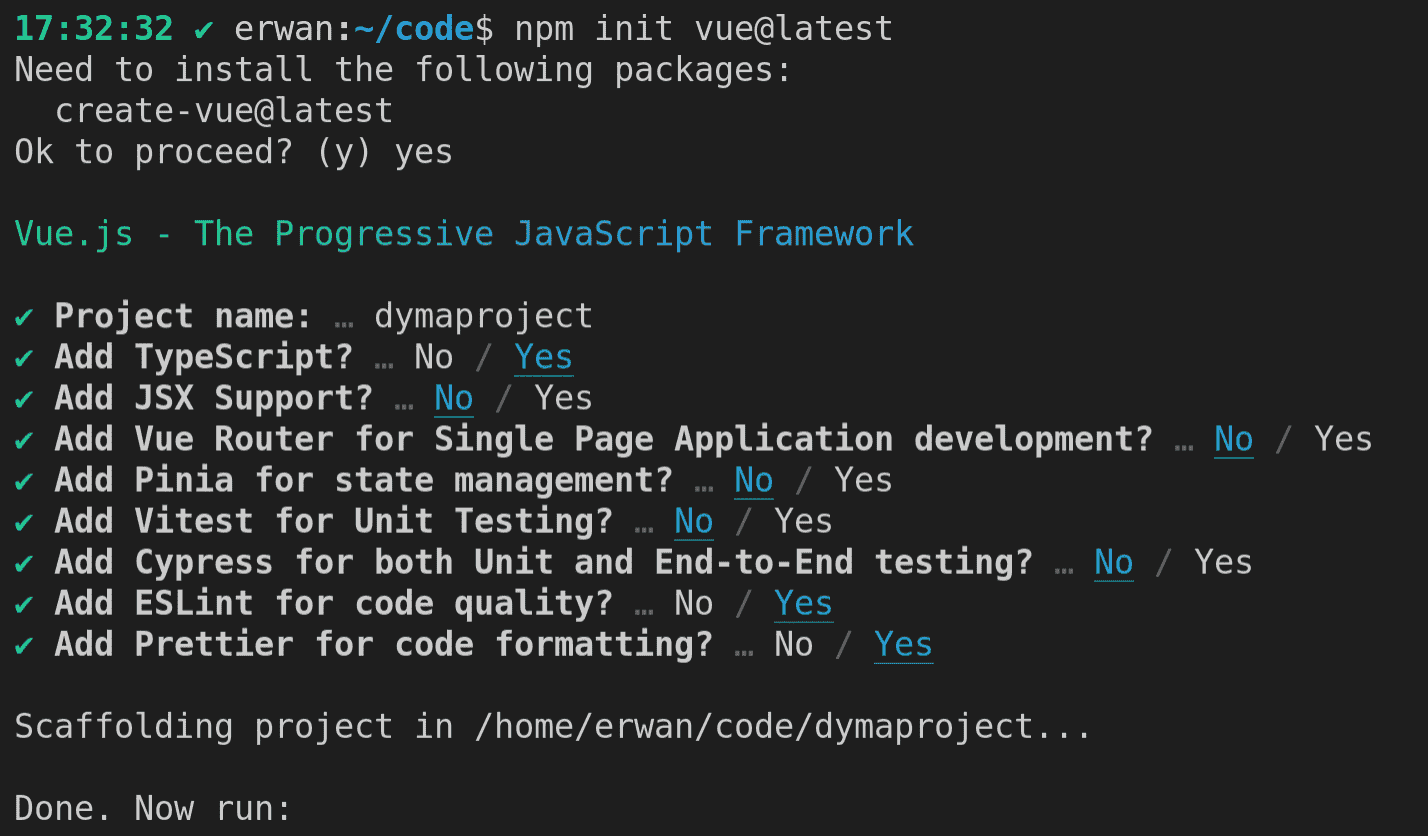
\includegraphics[width=10cm]{images/image04.png}
\end{center}



\end{document}

